\chapter{\rtd\ and \ee\ tutorial for \dspic}

This small tutorial describes a set of steps needed to compile a
simple application that shows the main features of \ee\ and \rtd\ for
the \dspic\ platform.

This tutorial has been tested on a \flex\ board produced by Evidence
and Embedded Solutions and on a Microchip Explorer 16 development
board from Microchip.

We suppose the reader is familiar with the MPLAB IDE debug environment
provided by Microchip.

%
% Questo era il testo che avevo inserito nel manuale di pic30 e che ho poi rimosso
%
%% As the first thing, the user has to create an RT-Druid Project from
%% the Eclipse IDE. When creating a new project, the developer has the
%% possibility of choosing an already existing example to start from. As
%% an alternative, the developer can start a project from scratch.

%% The \rtd\ project basically contains the source code of the
%% application, plus a configuration file written using the OIL
%% Language. A graphical editor for the OIL language is also available to
%% simplyfy the writing of the OIL file. For more information about the
%% OIL file syntax and the graphical editor, please refer to the \rtd\
%% reference manual.

%% Once the application has been written, it can be compiled by giving
%% the ``Build Project'' command from the Eclipse IDE.

%% The command basically asks \rtd\ to generate the \ee\
%% configuration code from the OIL file, and after that to compile the
%% application using the \file{makefile} generated by \rtd.

%% Once compiled, a coff image is obtained, which can be loaded inside
%% the MPLab IDE to load and debug the software inside the target
%% microcontroller.

%-----------------------------------------------------------------
\chapter{Notes for Windows XP and Windows Vista users}
\label{ch:vista}
%-----------------------------------------------------------------

If you are using Windows, and especially if you are using Windows
Vista, please look carefully at the following warnings:

\begin{warning}
Do NOT install the Evidence package in a name containing spaces.
\file{c:/Evidence/Evidence} works.
\end{warning}

\begin{warning}
Do NOT install the Scilab package in a name containing spaces.
\file{c:/Evidence/scilab-4.1.2} works.
\end{warning}

\begin{warning}
If using Vista, be aware that directories like 
\file{c:/Programmi}, \file{c:/Users/Documenti} are not REAL 
directories but are aliases. DO NOT USE THEM. Put your \rtd\ 
workspace under \file{c:/Users/yourusername/workspace}.
\end{warning}

\begin{warning}
Please install cygwin into its default directory, \file{c:/cygwin}.
\end{warning}

\begin{warning} Also if from the Windows Vista Explorer your Microchip
compiler seems to be installed under
\file{c:/Programmi/Microchip/...}, please remind to specify the REAL
pathmname. In particular, \file{c:/Programmi} DOES NOT EXISTS, whereas
the correvct name is \file{c:/Program Files}.  \end{warning}


\chapter{Installing \ee\ and \rtd\ on Microsoft Windows}
\label{cha:installing}

This chapter will guide the developer to the installation procedure of
\ee\ and \rtd\ for the \dspic\ platform.

The installation of \ee\ and \rtd\ is composed by the following
packages:
\begin{itemize}
\item The Eclipse development environment, which is used by \rtd\ to
  provide the basic development environment for \ee\ applications.
\item The Eclipse environment is based on the Java platform, so that
  a working Java Runtime Environment must be present for using \rtd.
\item The \rtd\ plugins, which provide the code generation for \ee\
  for Eclipse.
\item The \ee\ source code.
\item The Microchip MPLAB IDE.
\item The Microchip C30 Compiler.
\item A version of the Microchip C30 compiler recompiled from the GCC
  sources, which enables basic C language compilation without the need
  to buy the full fledged Microchip C30 Compiler.
\item A set of examples for the \dspic\ Platform, which can be used to
  compile a first set of running examples for the Evidence/Embedded
  Solutions \flex\ board, the Microchip Explorer 16 board, and
  others. These applications are organized in ``templates'', available
  at project creation.
\item A subset of the Cygwin environment \cite{cygwin}, including
  a set of utilities like \file{make}, \file{gawk}, and few others, which
  are used during the compilation process of an \ee\ application.
\end{itemize}

To install the software, execute the following steps:

\begin{enumerate}

\item Install your favourite Java runtime environment, which is needed
  to run \rtd; in fact, \rtd\ is a plugin of the Eclipse editor, which
  requires Java to be executed.

\item Install the latest version of the Microchip MPLAB IDE; you can
  use the default install directory. At the end of the install
  process, accept the system reboot.
  
\item Install the Microchip C30 Compiler, available from the Microchip
  web site.  Even in this case, you can use the default install
  directory. When it is asked to change the default environment,
  please do accept.

\item Run the \ee\ and \rtd\ installer.

\item The installer will prompt a list of packages which can be
  installed. Select all the packages you wish to install and
  continue the installation procedure (see Figure \ref{fig:installer-options}).
%
\begin{figure}[htb]
\begin{center}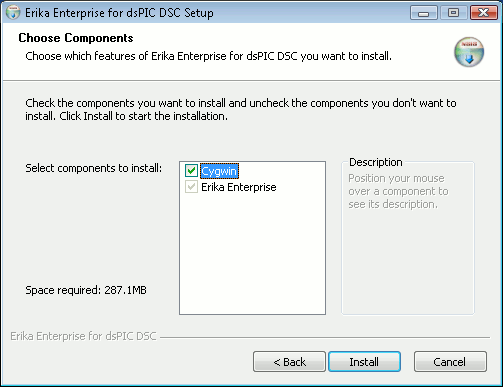
\includegraphics[
  width=8cm, bb=0 0 503 387]{images/installer_options.png}\end{center}
\caption{This screenshot shows the dialog box with the available install packages.}
\label{fig:installer-options}
\end{figure}

%\item The install package may not contain the MPLAB IDE in the list of
%  the available packages to install, as in the picture of Figure 
%  \ref{fig:installer-options}. If so, please download and install the
%  MPLAB IDE from the Microchip website.

%\item The install package may not contain the Microchip C30 Compiler
%  in the list of the available packages to install, as in the picture 
%  of Figure \ref{fig:installer-options}. If you need the Microchip C30
%  Compiler, please download or buy the appropriate package from the
%  Microchip website.

  \begin{note}
    The \ee\ install package provides a version of the Microchip C30
    compiler recompiled from the GCC sources made available from
    Microchip. Although that compiler is able to compile \ee\
    applications, it does not include Microchip include files and
    libraries which are only distributed with the Microchip package.
  \end{note}

\item The installer will ask for a destination directory. If possible, 
  please use \file{c:/Evidence/Evidence} (see Figure
  \ref{fig:installer-dir}).
%
\begin{figure}[htb]
\begin{center}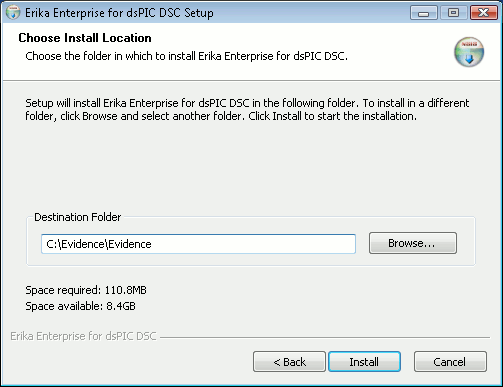
\includegraphics[
  width=8cm, bb=0 0 503 387]{images/installer_dir.png}\end{center}
\caption{This screenshot shows the preferred destination dir for installing \ee.}
\label{fig:installer-dir}
\end{figure}


\item At this point, please check the {\em first} line of the file
  \file{evidencedir\\bin\\mymake_cygwin.bat} (where \file{evidencedir}
  is the directory you chose during the installation). For example,
  if Cygwin is installed inside \file{C:\\cygwin}, then the first line
  of the file should look like the following one:
\begin{lstlisting}
@set EE_BASH_PATH=C:\cygwin\bin\bash
\end{lstlisting}
  ...that is, the line contains the correct path to the
  \file{bash.exe} file in your Cygwin installation. If you accepted
  the default settings, the correct pathname should be
  \file{C:\\cygwin\\bin\\bash} as specified in the example before.
  \begin{note}
    We ask to perform this check because it seems that on some Windows
    machines the Cygwin installer does not correctly set the registry
    keys used by the \ee\ installer.
  \end{note}
\end{enumerate}

The rest of this tutorial supposes that the Microchip MPLAB IDE is
installed within the \file{C:\\Programmi\\Microchip} directory and
that, consequently, the GNU Assembler for \dspic\ is installed within
\file{C:\\Programmi\\Microchip\\MPLAB ASM30 Suite\\bin}. Please note
that these values may be different from the settings you have chosen
on your machine. Please also read the chapter with the Windows Vista
recommendations.

\chapter{First \rtd\ startup and configuration}

After all the required packages have been installed, you are ready to
start \rtd\ for the first time.

Please follow the next steps:

\begin{enumerate}
\item As the first step, run the Eclipse IDE from the Evidence menu
  inside the Start menu of your Windows machine, choosing 
  \file{Start/Programs/Evidence/RT-Druid}.
  
\item A dialog box will appear, asking to choose the right
  workspace (see Figure \ref{fig:select-workspace}). 
  Leave the default workpackage directory
  as it is, and proceed by pressing ``OK''.
%
\begin{figure}[htb]
\begin{center}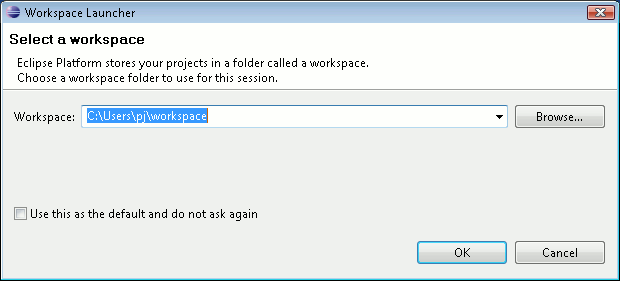
\includegraphics[
  width=8cm, bb=0 0 620 281]{images/select_workspace.png}\end{center}
\caption{This screenshot shows the
dialog box for the choice of the current workspace directory.}
\label{fig:select-workspace}
\end{figure}

\begin{warning}
The workspace pathname MUST NOT contain any blank space, otherwise 
\ee\ and \rtd\ may not work properly.
\end{warning}

\begin{note}
If you are using Windows Vista, then the workspace directory \file{c:/Users/<username>/workspace} works.
\end{note}

% ---

\item
  The Eclipse Welcome screen appears, like in Figure \ref{fig:welcome}.
%
\begin{figure}[htb]
\begin{center}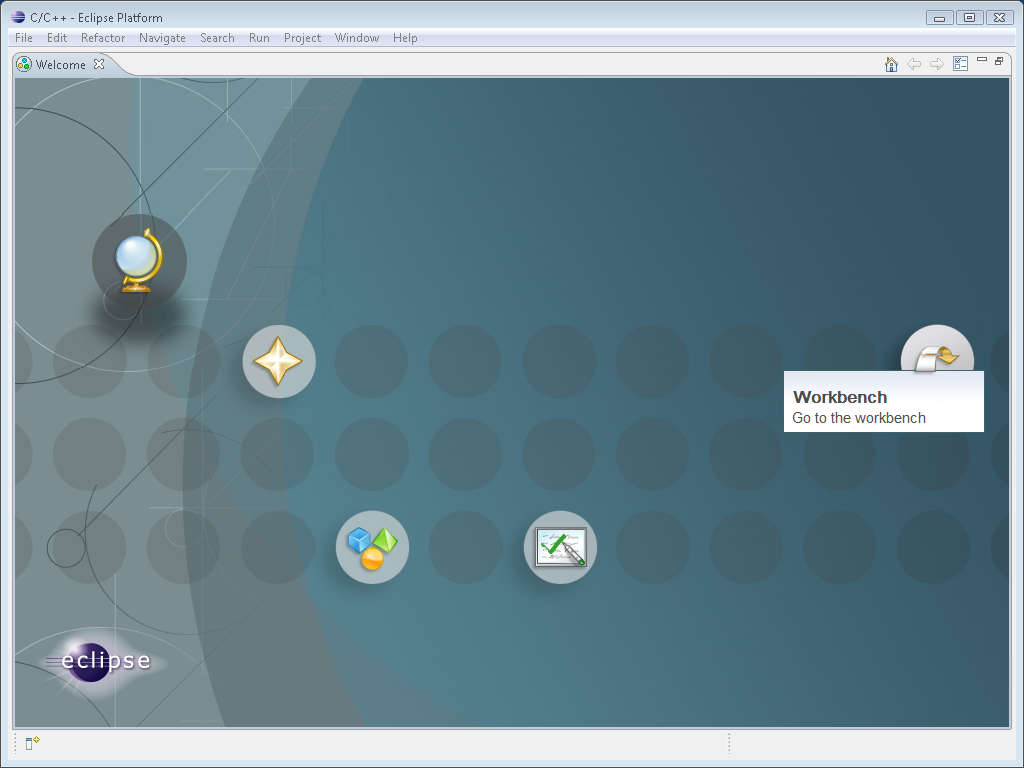
\includegraphics[
  width=12cm, bb=0 0 1024 768]{images/welcome.png}\end{center}
\caption{The Eclipse Welcome screen.}
\label{fig:welcome}
\end{figure}

\item
Before being able to correctly build your application, you should set
the path to the Microchip C30 compiler and the MPLAB ASM30 assembler
programs. For doing so, please go to the ``Preference'' menu, as shown
in Figure \ref{fig:preferences-menu}, and find the
``RT-Druid/Oil/PIC30 Configurator'' form as depicted in Figure
\ref{fig:preferences-pic30}.  The first textbox, labeled \const{Gcc
path}, refers to the installation directory of the Microchip C30
compiler. The second textbox, labeled \const{Asm path}, refers to the
installation directory of the ASM30 assembler provided with the MPLAB
IDE.

\begin{warning}
The install directories specified in the two textboxes of Figure
\ref{fig:preferences-pic30} does {\em not} include the \file{bin}
directory! 

That is, \file{c:\\Programmi\\Microchip\\MPLAB C30} is correct, wheras
\file{c:\\Programmi\\Microchip\\MPLAB C30\\bin} is not.
\end{warning}

\begin{warning}
The install directory of the assembler refers to the assembler
provided with MPLAB IDE and {\em not} the assembler provided with the
C30 compiler. The reason is that the directory is used to call the
assembler and {\em also} to copy the \file{crt0.s} file, which has a
different position in the two assemblers distributions made by
Microchip.
\end{warning}

\begin{warning}
If you are using a Student Editon of the Microchip C30 compiler which
has an {\bf expired license}, please check the ``Use EE gcc to resolve
dependencies'' checkbox in Figure \ref{fig:preferences-pic30}.
\end{warning}

  \begin{figure}[htb]
\begin{center}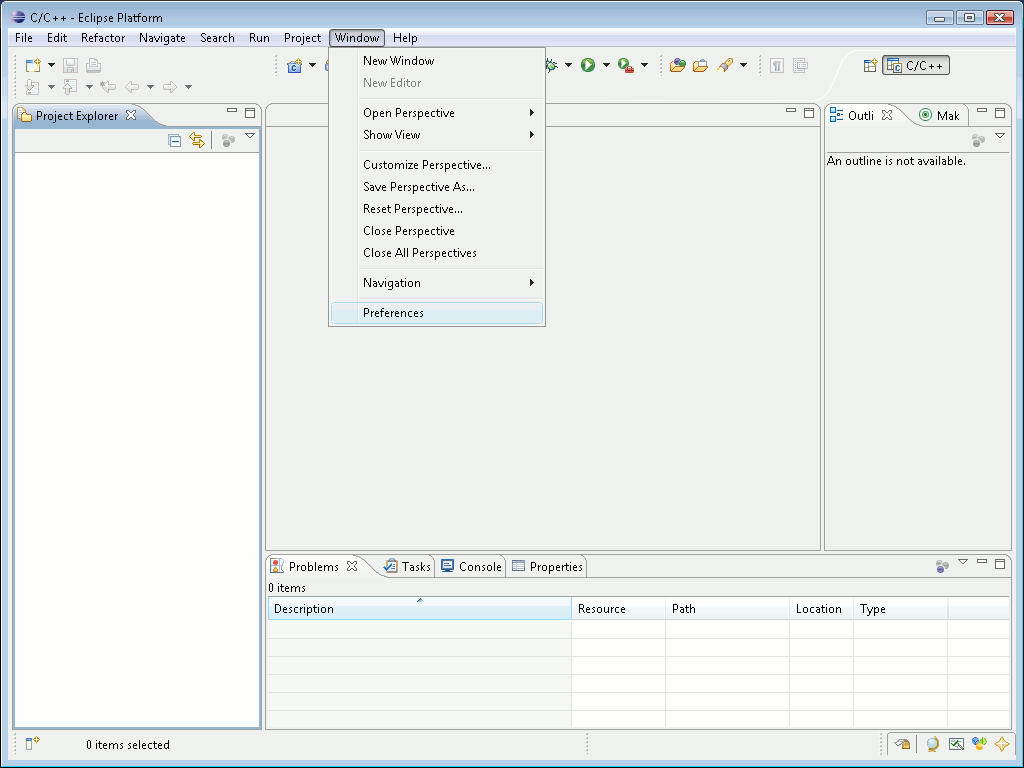
\includegraphics[
  width=8cm, bb=0 0 1024 768]{images/preferences_menu.png}\end{center}
\caption{Go to the ``Preference'' menu.}
\label{fig:preferences-menu}
\end{figure}

\begin{figure}[htb]
\begin{center}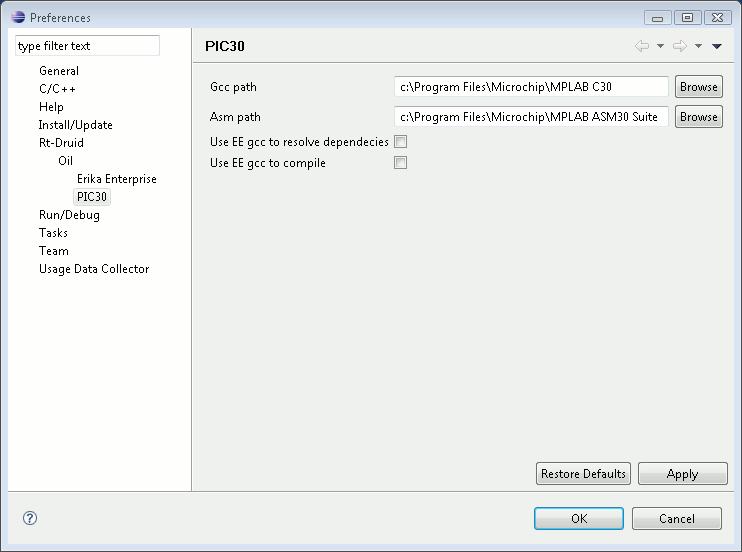
\includegraphics[
  width=8cm, bb=0 0 742 552]{images/preferences_pic30.png}\end{center}
\caption{Select paths for compiler and assembler.}
\label{fig:preferences-pic30}
\end{figure}

% ---

\item
  Before creating and building your application, please deselect the
  ``Build Automatically'' flag inside the ``Project'' menu, as shown
  in Figure \ref{fig:build-automatically}.
%
\begin{figure}[htb]
\begin{center}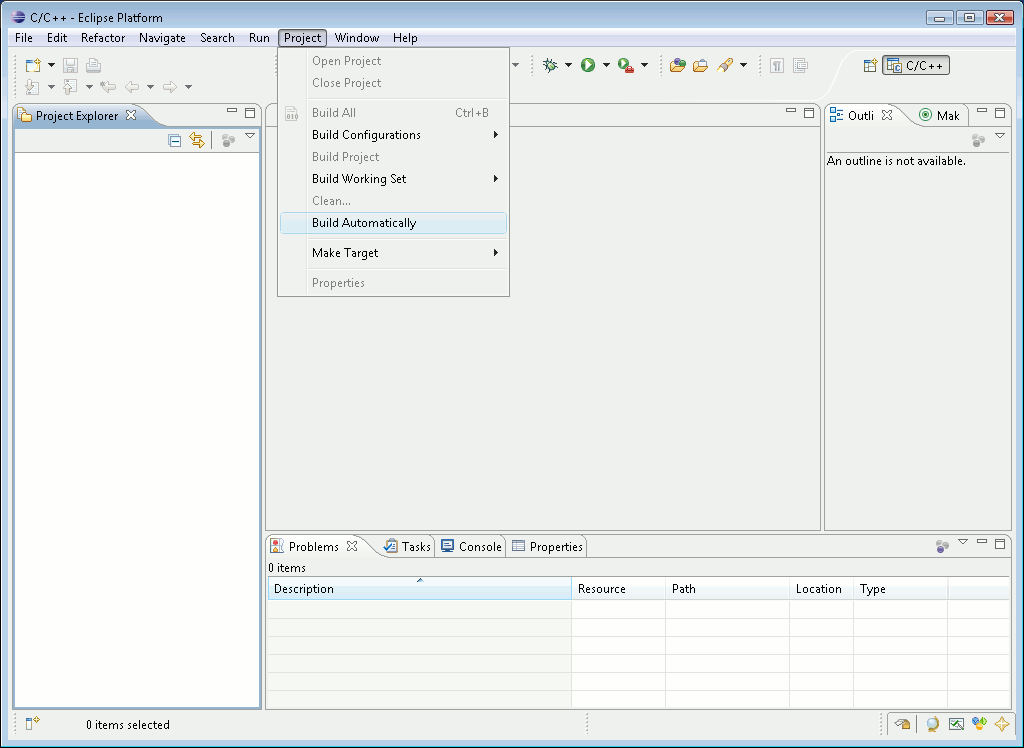
\includegraphics[
  width=8cm, bb=0 0 1024 748]{images/build_automatically.png}\end{center}
\caption{Deselect the ``Build Automatically'' flag in the ``Project'' menu.}
\label{fig:build-automatically}
\end{figure}

% ---

% /toOl:
%\item
%  \nb{bla bla bla. bisogna descrivere: la selezione del workpackage, la configurazione delle opzioni di base}

\end{enumerate}

\chapter{Compiling your first \ee\ demo for \dspic}


You are now ready to compile your first \ee\ demo. Please execute the
following steps:

\begin{enumerate}

\item
  Please select ``New Project'', then ``RT-Druid Oil and c/c++
  Project'' from the ``File menu'', as in Figure
  \ref{fig:new-project}.
%
\begin{figure}[htb]
\begin{center}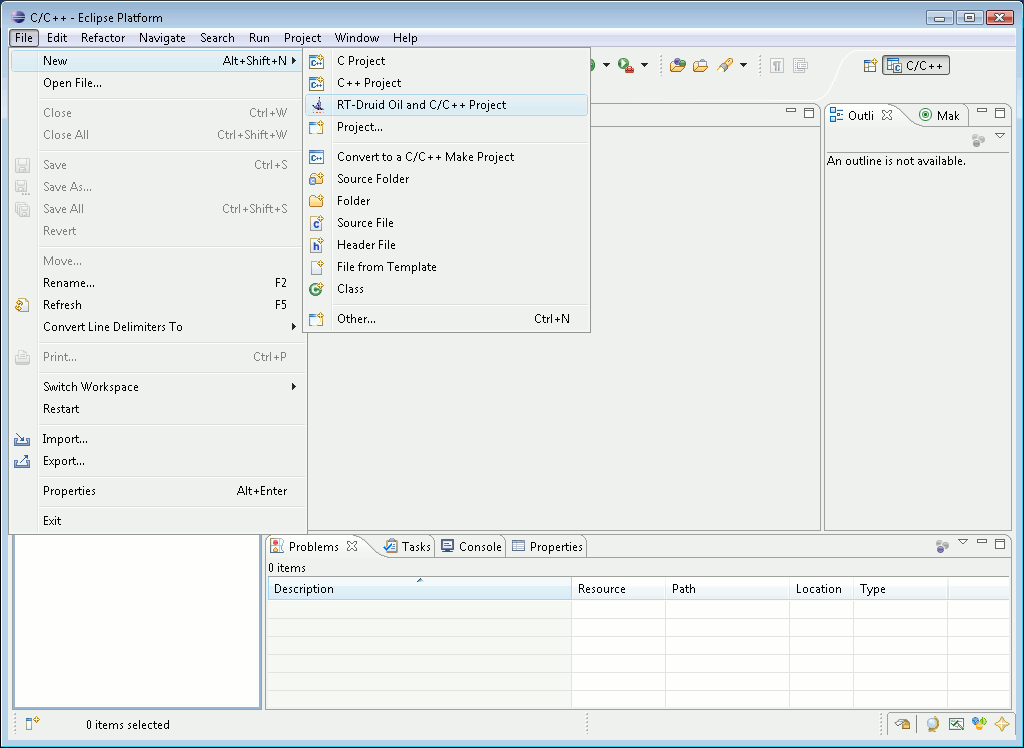
\includegraphics[
  width=12cm, bb=0 0 1024 748]{images/newproject.png}\end{center}
\caption{Select ``New project'' from the ``File'' menu.}
\label{fig:new-project}
\end{figure}

\item
  A Dialog box appear. Please select a template for the new project,
  as in Figure \ref{fig:new-project2}.
%
\begin{figure}[htb]
\begin{center}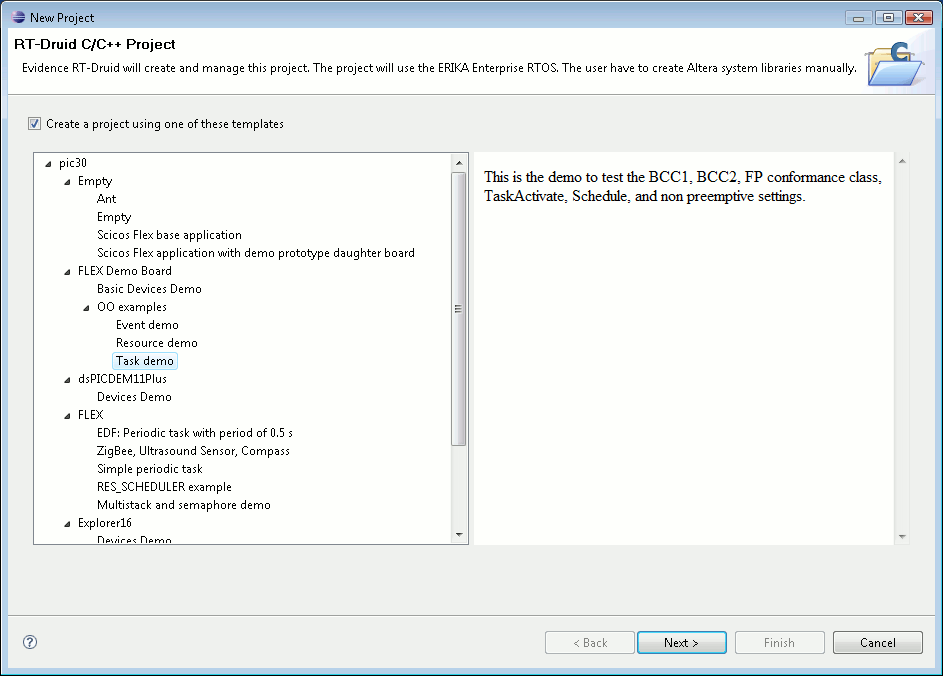
\includegraphics[
  width=8cm, bb=0 0 943 676]{images/newproject2.png}\end{center}
\caption{Select a template for your project.}
\label{fig:new-project2}
\end{figure}

\item
  Press ``Next''.

\item
  Insert the name of the new project. Please type \const{taskdemo}
  (you can choose other names of course). Please see Figure
  \ref{fig:projectname}. Press the ``Finish'' button.
%
\begin{figure}[htb]
\begin{center}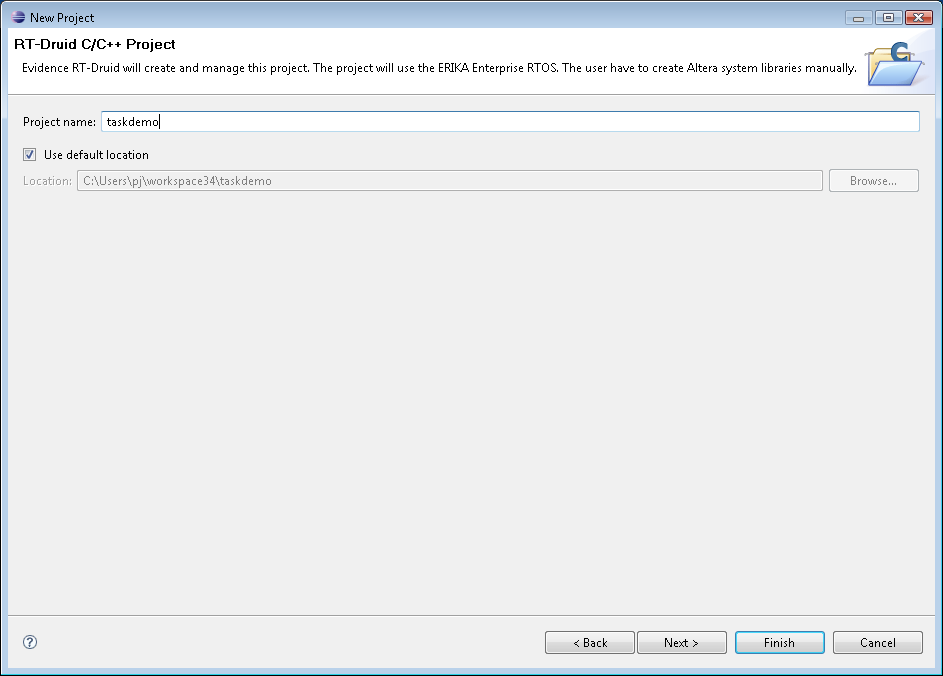
\includegraphics[
  width=8cm, bb=0 0 943 676]{images/projectname.png}\end{center}
\caption{Type a name for the new project.}
\label{fig:projectname}
\end{figure}

%% \item
%% % /toOl:
%% % \nb{capire se ci sara una licenza!}
%%   If the \rtd\ version you are using requires a valid license, and if
%%   it is the first time you run the Evidence plugins on the Eclipse
%%   installation, a Dialog box asking a valid license will appear. The
%%   dialog box looks like the one in Figure
%%   \ref{fig:license-welcome}. Press the ``Install license'' button to
%%   provide a valid license. If you do not have a valid license, please
%%   contact the Evidence technical support at
%%   \const{support@evidence.eu.com}.
%% %
%% \begin{figure}[htb]
%% \begin{center}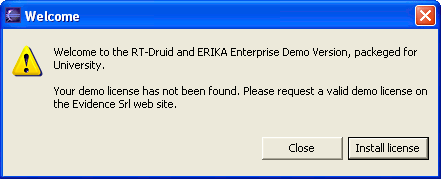
\includegraphics[
%%   width=8cm, bb=0 0 441 179]{images/license_welcome.png}\end{center}
%% \label{fig:license-welcome}
%% \caption{The dialog box asking for the Evidence License file.}
%% \end{figure}

%% \item
%%   The system asks for a valid license (see Figure
%%   \ref{fig:license-installer}). Please press the ``Browse button'' to
%%   select the license file on the filesystem.
%% %
%% \begin{figure}[htb]
%% \begin{center}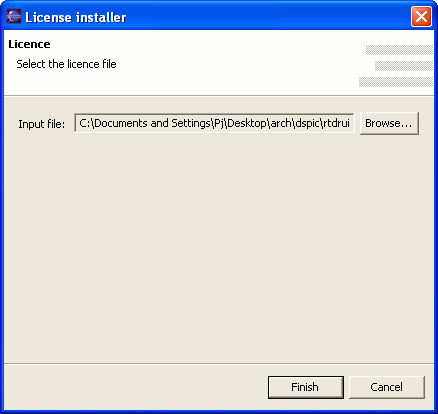
\includegraphics[
%%   width=8cm, bb=0 0 438 414]{images/license_installer.png}\end{center}
%% \label{fig:license-installer}
%% \caption{Please select a valid license file.}
%% \end{figure}

%% \item
%%   If the license file specified is valid, a message box like the one
%%   in Figure \ref{fig:remainingdays} will appear, informing you about
%%   the type of license selected. Press ``Close'' to close the message
%%   box. In the future, you can check the status of your license file by
%%   clicking on the ``Evidence License Manager'' item on the ``Help''
%%   menu. In that case, a Message box like Figure
%%   \ref{fig:license-manager} will appear.
%% %
%% \begin{figure}[htb]
%% \begin{center}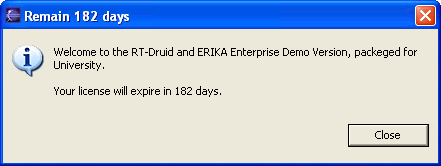
\includegraphics[
%%   width=8cm, bb=0 0 441 166]{images/remainingdays.png}\end{center}
%% \label{fig:remainingdays}
%% \caption{This window informs you about the type of license you selected.}
%% \end{figure}
%% %
%% \begin{figure}[htb]
%% \begin{center}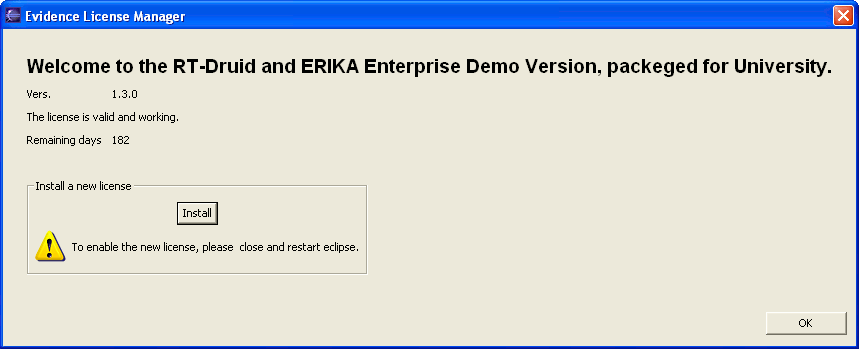
\includegraphics[
%%   width=8cm, bb=0 0 859 349]{images/license_manager.png}\end{center}
%% \label{fig:license-manager}
%% \caption{This window informs you about the type of license you selected.}
%% \end{figure}


%% \item
%%   We are now ready to import and compile your first example. Right
%%   click on the project name in the navigation bar, and select
%%   ``Import...'', like in Figure \ref{fig:importfilesystem}. Then,
%%   select ``Import Filesystem'' like in Figure
%%   \ref{fig:importfilesystem2}.  In the ``From directory'' textbox,
%%   type the name of the example directory you can find inside the \ee\
%%   install directory (in Figure \ref{fig:importfilesystem3}, inside
%%   \file{C:\\Programmi\\Evidence\\pic30\\} \file{examples\\pic30_oo_mono}); you
%%   can also select it using the ``Browse'' button to browse
%%   directories. Choose the directory name in the tree view on the left,
%%   selecting all the files on the right side. The ``Into Folder'' text
%%   box should point to the project you just created. Finally, select
%%   the checkbox ``Overwrite existing resources without warning'' and
%%   press Finish.

%% %
%% \begin{figure}[htb]
%% \begin{center}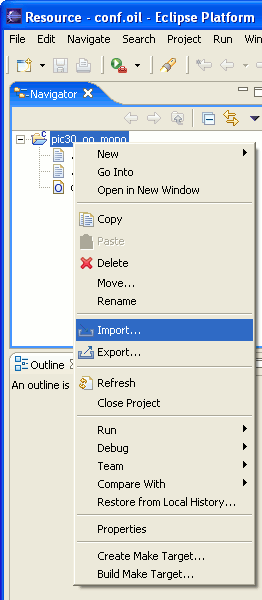
\includegraphics[
%%   width=4cm, bb=0 0 262 600]{images/import_filesystem.png}\end{center}
%% \label{fig:importfilesystem}
%% \caption{Importing an existing example inside the project.}
%% \end{figure}
%% %
%% \begin{figure}[htb]
%% \begin{center}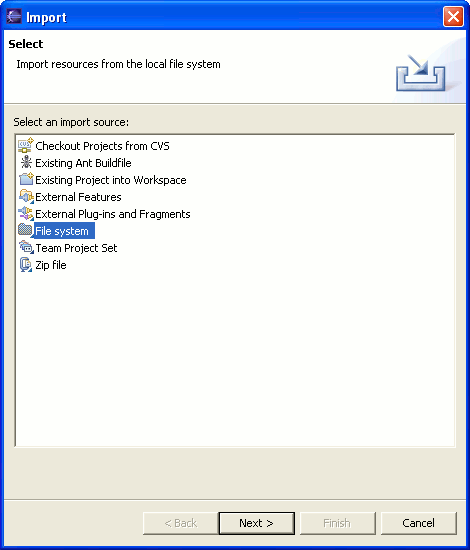
\includegraphics[
%%   width=8cm, bb=0 0 470 550]{images/import_filesystem2.png}\end{center}
%% \label{fig:importfilesystem2}
%% \caption{Selecting ``Importing Filesystem'' to copy an existing project inside the current project.}
%% \end{figure}
%% %
%% \begin{figure}[htb]
%% \begin{center}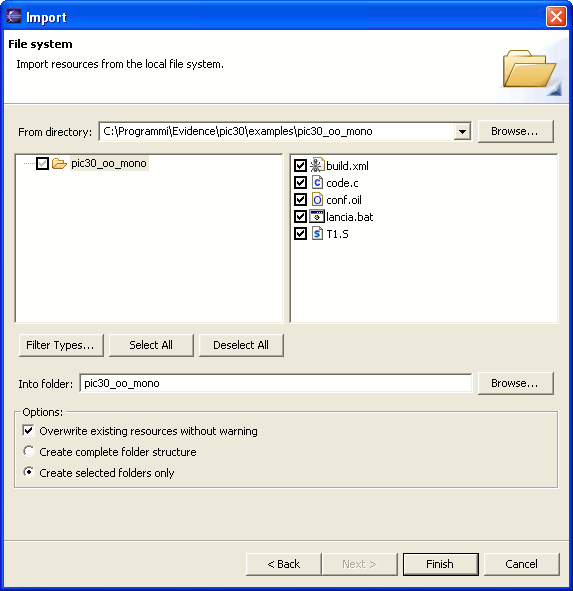
\includegraphics[
%%   width=8cm, bb=0 0 573 591]{images/import_filesystem3.png}\end{center}
%% \label{fig:importfilesystem3}
%% \caption{Importing the files inside the project.}
%% \end{figure}

%% \item
%%   The last step before building the demo implies the setup of the
%%   Eclipse CDT builder properties. Right-click on the Project name in
%%   the Eclipse Navigation bar, and choose ``Properties''. Click on the
%%   ``C/C++ Make Project'' tab, and be sure that: in the ``Build
%%   Command'' frame, ``Use default'' checkbox is not checked; ``Build
%%   command'' should point to the \file{installdir\\bin\\mymake.bat}
%%   executable, where {\em installdir} is the installation directory of
%%   the Evidence tools; in the ``Build Directory'' frame, the ``Build
%%   directory'' textbox should contain ``\\{\em projectname}\\Debug'',
%%   where {\em projectname} is the name of the project. See Figure
%%   \ref{fig:pic30-properties} for an example.
%% %
%% \begin{figure}[htb]
%% \begin{center}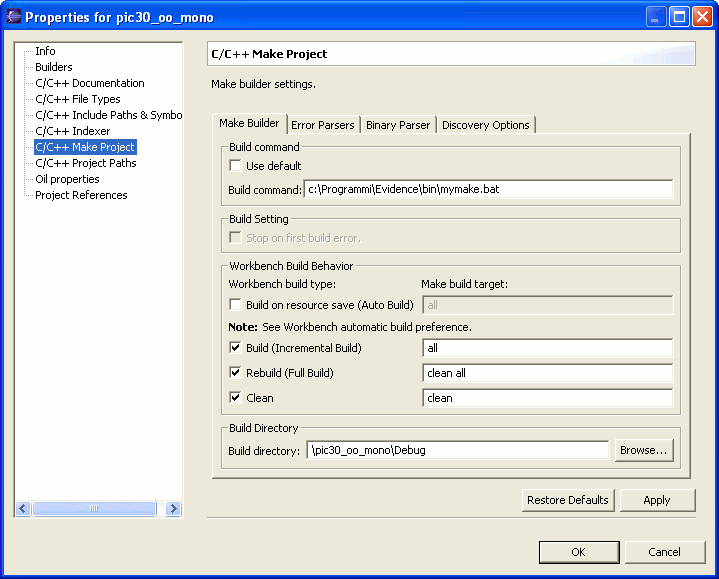
\includegraphics[
%%   width=8cm, bb=0 0 719 579]{images/pic30_properties.png}\end{center}
%% \label{fig:pic30-properties}
%% \caption{The CDT Make properties for the \rtd\ project.}
%% \end{figure}

\item
  We are now ready to build the demo. Right click on the project name
  in the Eclipse navigation bar, and choose ``Build
  Project''\footnote{``Build Project'' only appears if the ``Build
  Automatically'' flag is not selected in the ``Project'' menu.} (see
  Figure \ref{fig:build-project}).
%
\begin{figure}[htb]
\begin{center}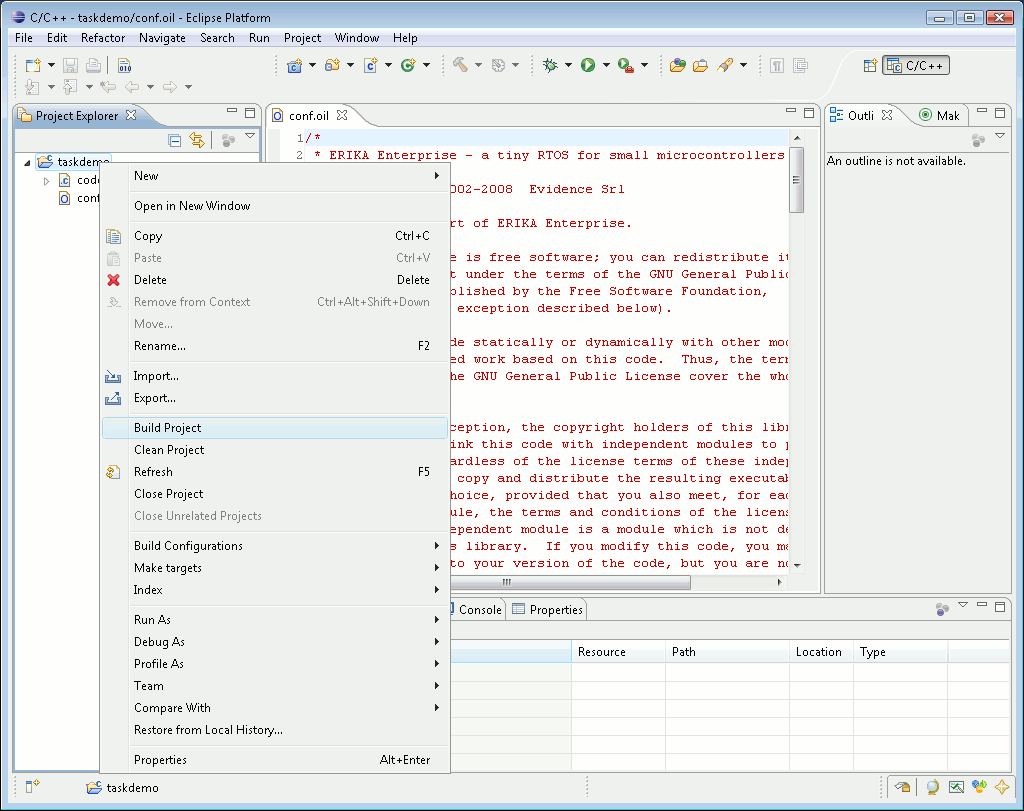
\includegraphics[
  width=10cm, bb=0 0 1024 811]{images/build_project.png}\end{center}
\caption{We are now able to build the project.}
\label{fig:build-project}
\end{figure}

\item
  Then, the compilation process starts as depicted in Figure
  \ref{fig:compiling}. Please note the message that appears when the
  compilation is successfull.
%
\begin{figure}[htb]
\begin{center}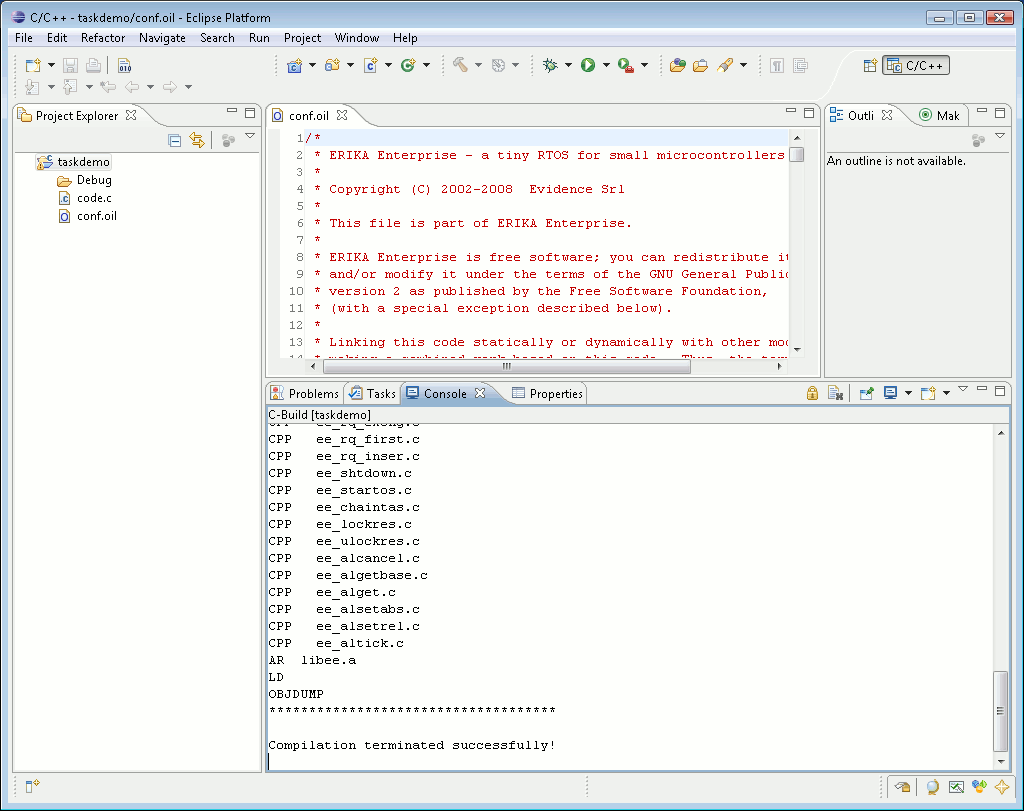
\includegraphics[
  width=10cm, bb=0 0 1024 811]{images/compiling.png}\end{center}
\caption{The compilation process.}
\label{fig:compiling}
\end{figure}

\begin{note}
  If the error depicted in Figure \ref{fig:mymake_cygwin_error} appears (meaning
  that \file{mymake_cygwin.bat} is unable to find a file), then please
  follow the instructions at the last point of Chapter
  \ref{cha:installing}.
\end{note}
%
\begin{figure}[htb]
\begin{center}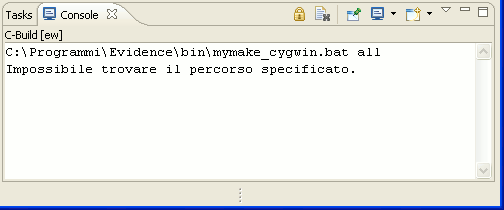
\includegraphics[
  width=10cm, bb=0 0 504 210]{images/mymake_cygwin_error.png}\end{center}
\caption{An error that shows up on some Windows machines. Please check the \file{mymake_cygwin.bat} file as explained in the last point of Chapter \ref{cha:installing}.}
\label{fig:mymake_cygwin_error}
\end{figure}

\item At the end of the compiling process you will be able to find a
  file named `\file{pic30.cof} inside the \file{Debug} directory
  inside the project, as shown in Figure \ref{fig:cof-file}.
%
\begin{figure}[htb]
\begin{center}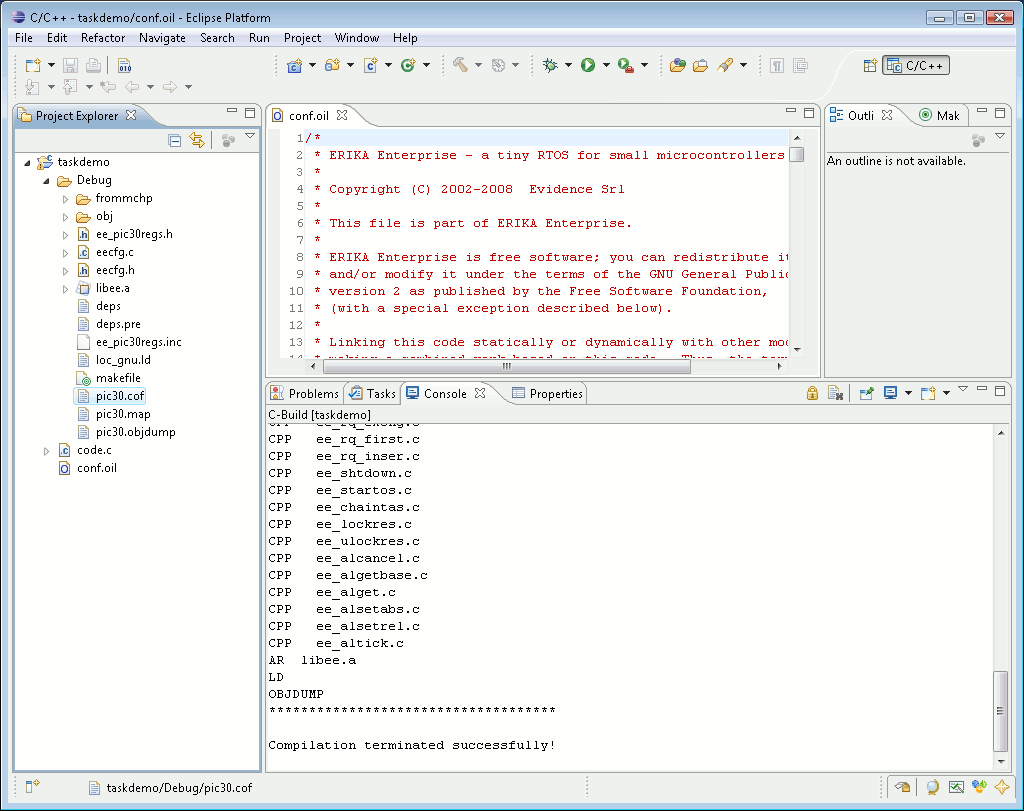
\includegraphics[
  width=10cm, bb=0 0 1024 811]{images/cof_image.png}\end{center}
\caption{The output file is ready to be programmed on the target board.}
\label{fig:cof-file}
\end{figure}

  
\item
  You are now ready to import the produced COFF file inside Microchip
  MPLAB IDE. To do that, open MPLAB IDE as in Figure \ref{fig:mplab1}.
%
\begin{figure}[htb]
\begin{center}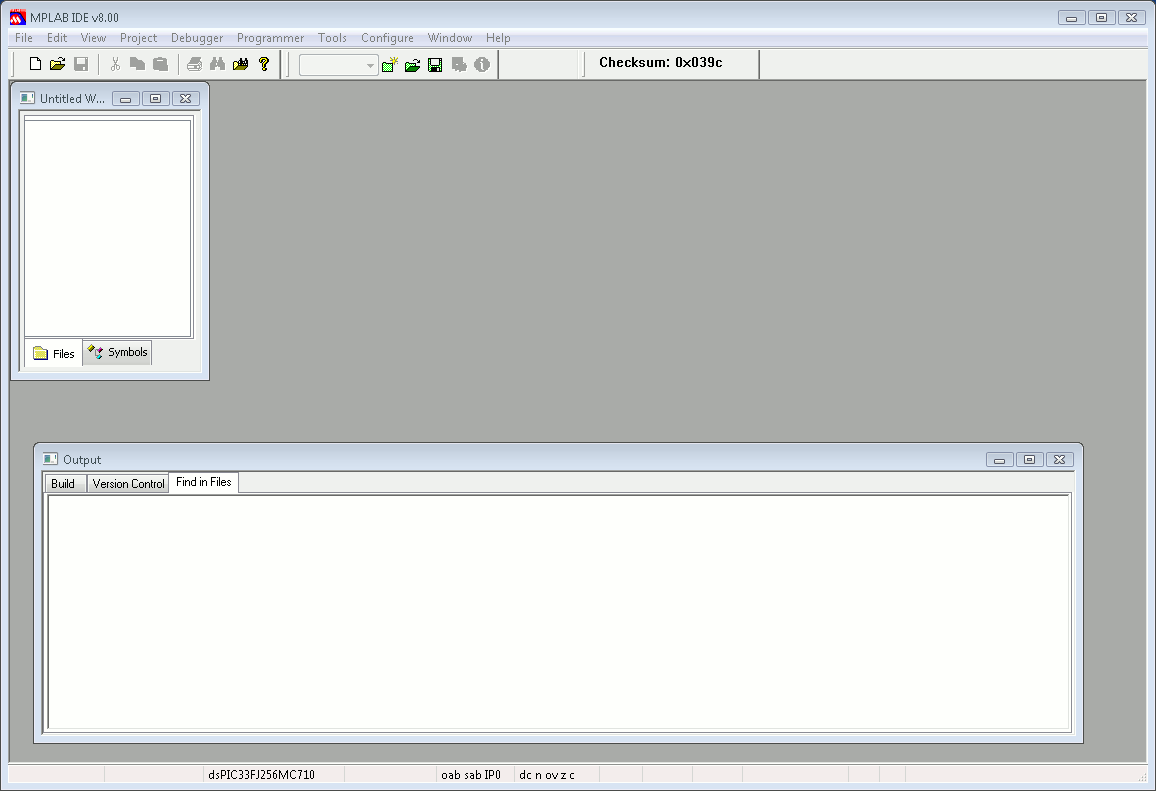
\includegraphics[
  width=12cm, bb=0 0 1156 791]{images/mplab1.png}\end{center}
\caption{The Microchip MPLAB IDE.}
\label{fig:mplab1}
\end{figure}

\item
  Choose ``Import...'' from the ``File'' menu, as in Figure \ref{fig:mplab2}.
%
\begin{figure}[htb]
\begin{center}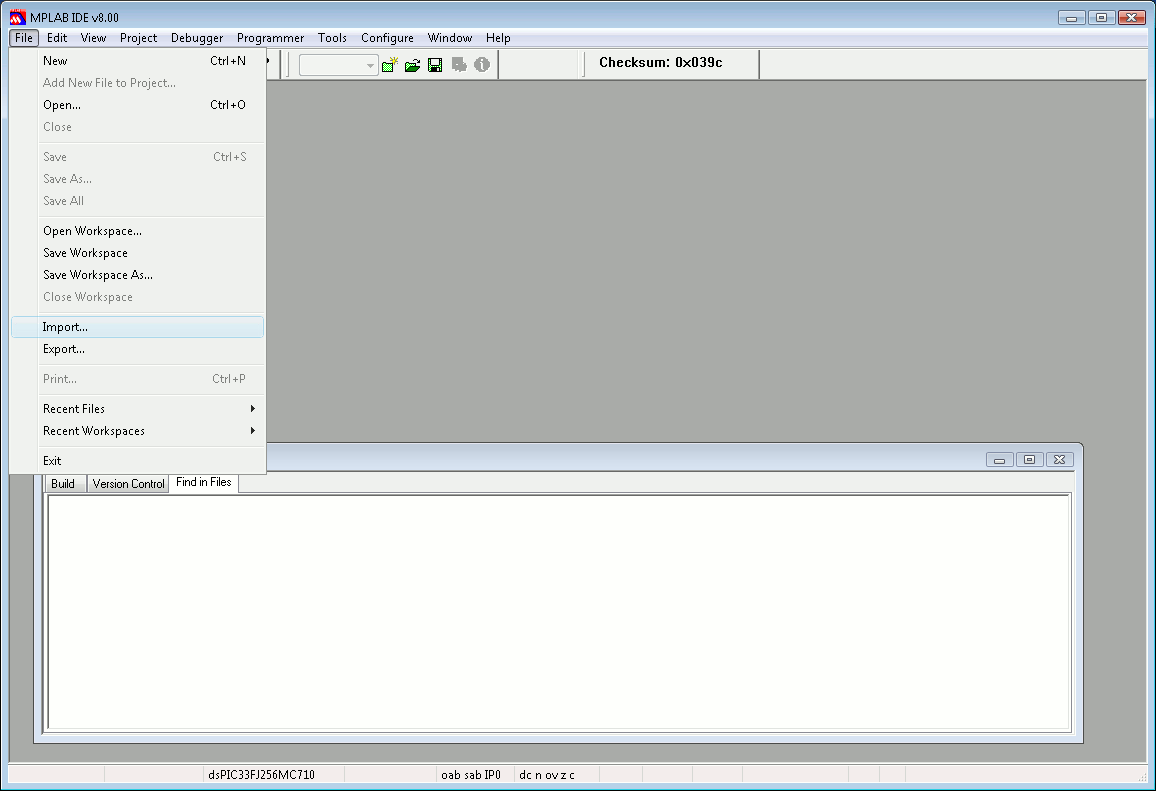
\includegraphics[
  width=12cm, bb=0 0 1156 791]{images/mplab2.png}\end{center}
\caption{Choose ``Import...'' from the ``File'' menu to import the coff file produced in Eclipse.}
\label{fig:mplab2}
\end{figure}

\item
  A dialog box appear. Please select the \file{pic30.cof} file that
  has been produced by the compilation process in Eclipse, as shown in
  Figure \ref{fig:mplab3}. You can find that file inside the Eclipse
  workspace you selected at the beginning in Figure
  \ref{fig:select-workspace}. In this example, the file is stored
  inside the directory
  \file{c:\\Programmi\\Evidence\\eclipse\\workspace\\} \file{pic30_oo_mono\\Debug}.
%
\begin{figure}[htb]
\begin{center}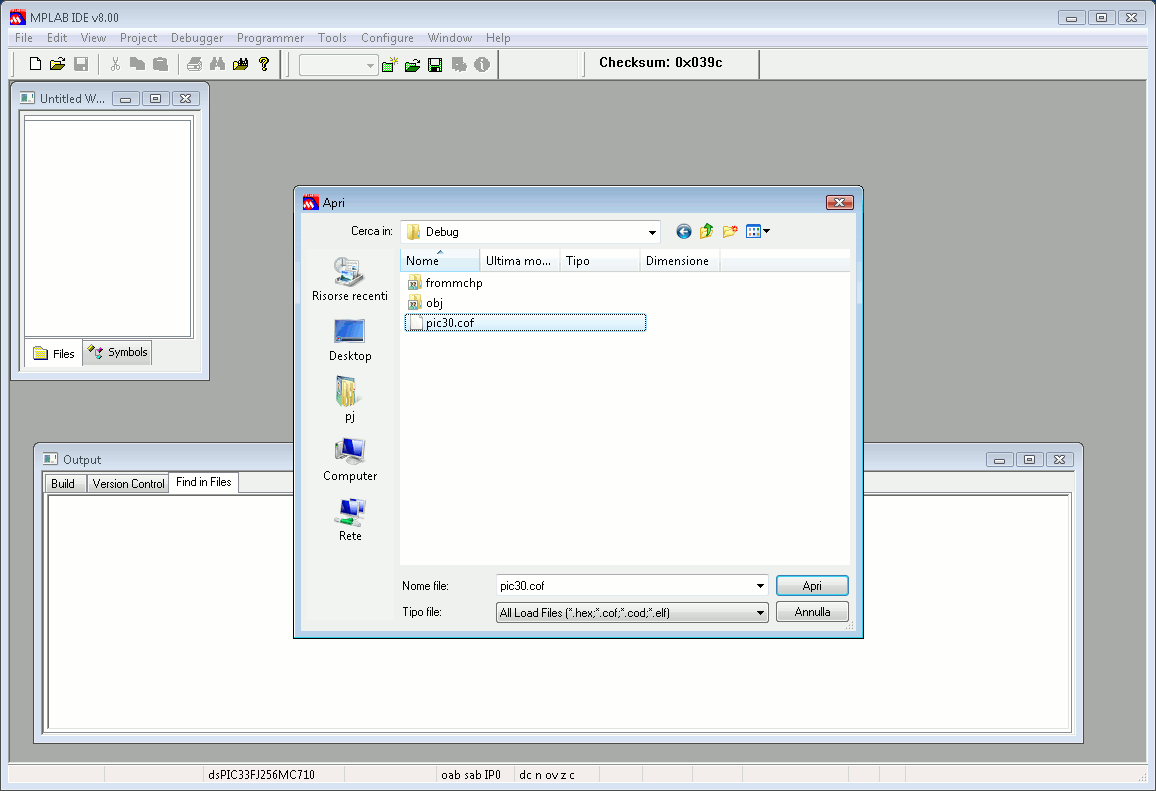
\includegraphics[%
  width=12cm, bb=0 0 1156 791]{images/mplab3.png}\end{center}
\caption{Select the COFF file you want to import.}
\label{fig:mplab3}
\end{figure}

\item
  You have now imported the COFF file inside MPLAB IDE. There is no
  need to create a MPLAB IDE Project, because the compilation process
  is handled by Eclipse. Figure \ref{fig:mplab4} shows the
  ``Disassembly Listing'' and the ``Program Memory'' window. Please
  note that MPLAB IDE correctly recognizes the debug symbols of the source
  code produced inside Eclipse.
%
\begin{figure}[htb]
\begin{center}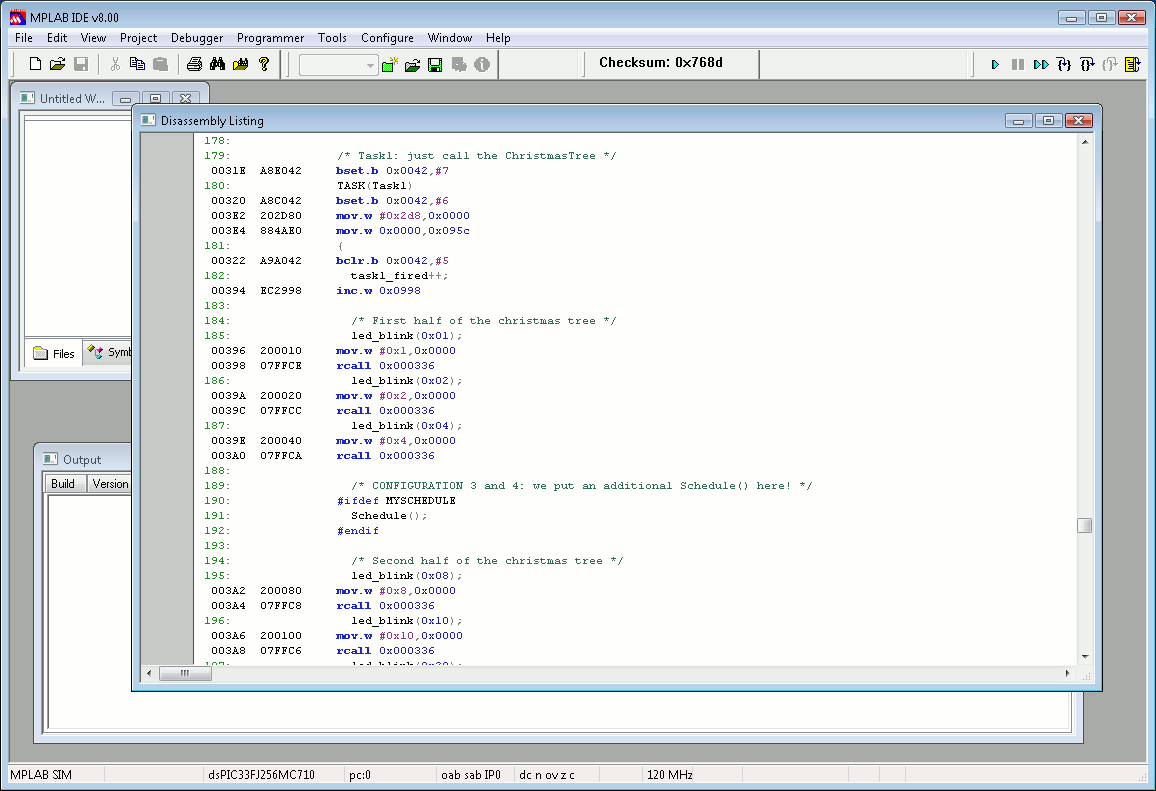
\includegraphics[
  width=12cm, bb=0 0 1156 791]{images/mplab4.png}\end{center}
\caption{Debug symbols are correctly recognized.}
\label{fig:mplab4}
\end{figure}

\item
  You can now start debugging the demo application using MPLAB IDE.
\end{enumerate}

Figure \ref{fig:explorer16running} shows the Explorer 16 board with the 
running \file{pic30\\explorer16\\Devices Demo} demo application, which uses the
Explorer 16 onboard devices to monitor and display the environment temperature.

\begin{figure}[htb]
\begin{center}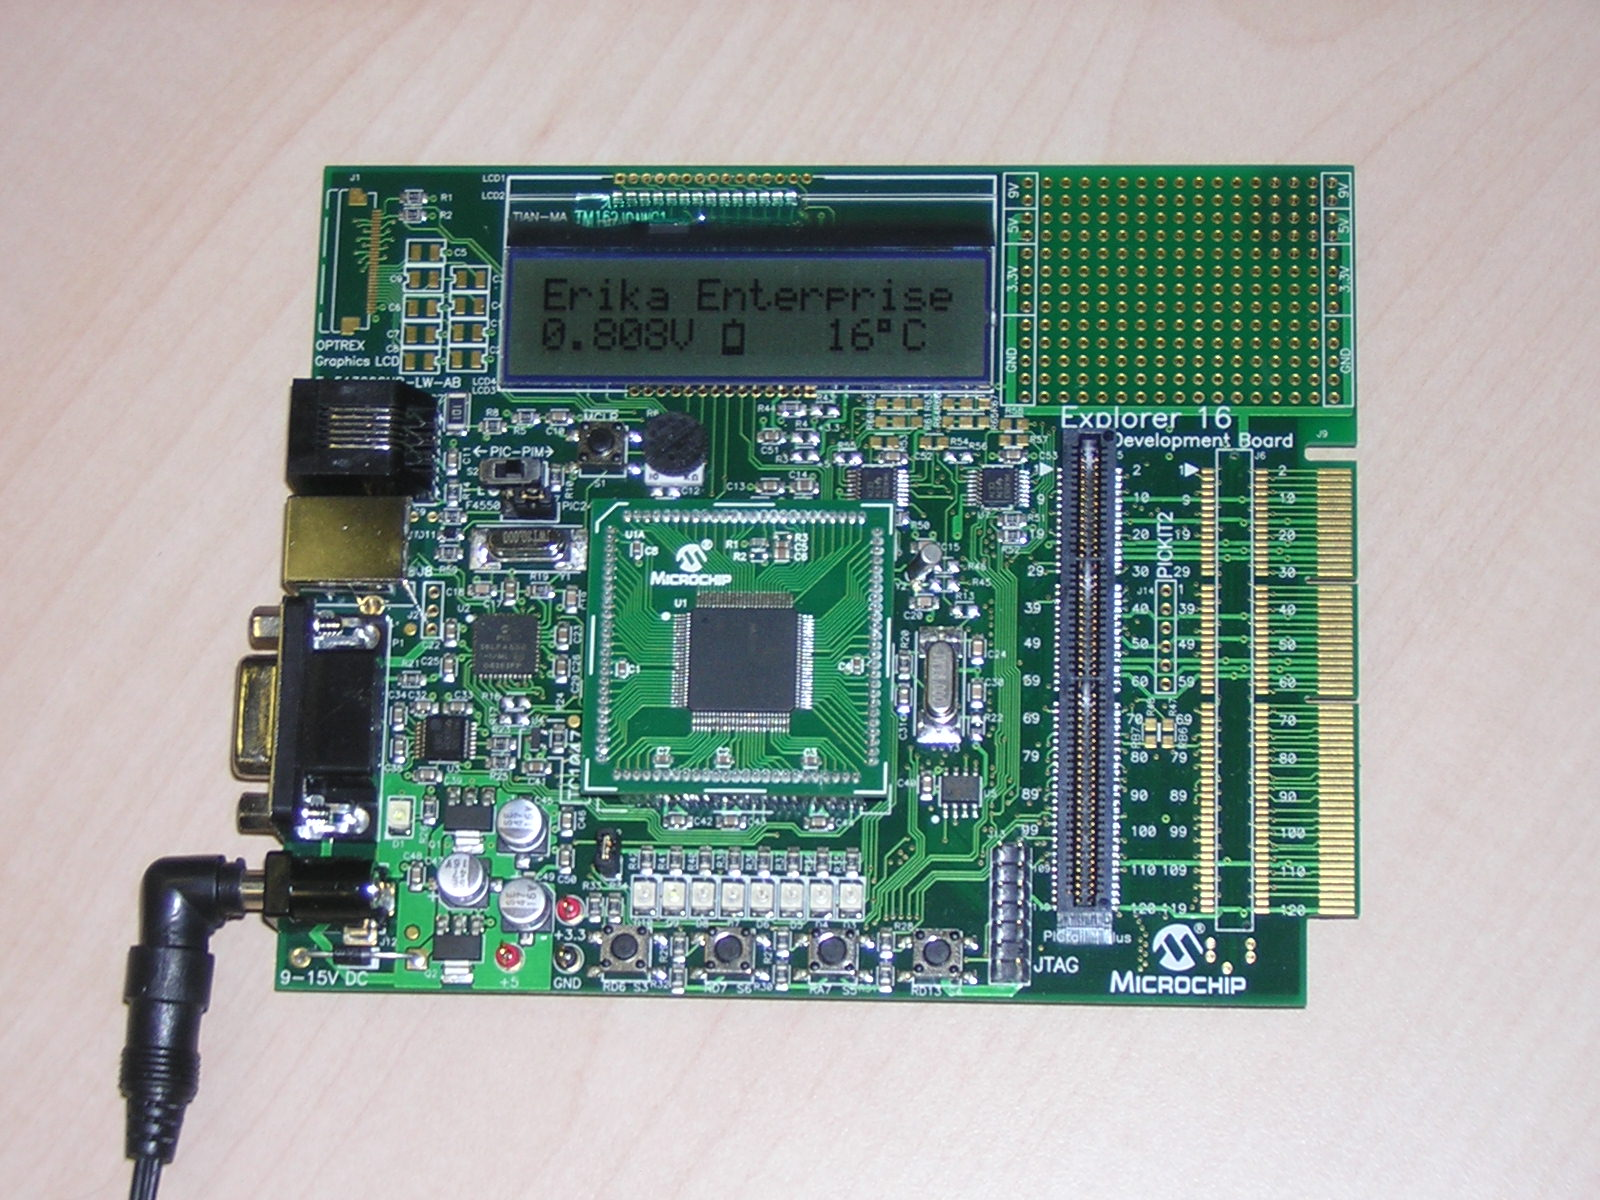
\includegraphics[
  width=12cm, bb=0 0 1600 1200]{images/explorer16running.jpg}\end{center}
\caption{The Explorer 16 board with the running demo program.}
\label{fig:explorer16running}
\end{figure}

\begin{note}
If you get an MPLAB IDE error like the following:

\begin{lstlisting}
ICDWarn0015: Program memory has changed since 
last program operation?
Continue with Debug operation?
Running Target
ICD0083: Debug:  Unable to enter debug mode.  
Please double click this
message for more information.
\end{lstlisting}

Please be sure that you entered the debug mode and programmed the device {\em from the Debugger Mode} and not from the Programmer Mode.
\end{note}

\begin{note}
If you are using a \flex\ board, please remember to set the device
correctly uinder the ``Configure / Select device...'' menu of
MPLABIDE.

The correct settings for the dsPIC on the \flex\ Full and the \flex\
Light is shown in Figure \ref{fig:mplab-selectdevice-dspic}. The
correct settings for the PIC18 on the \flex\ Full is shown in Figure
\ref{fig:mplab-selectdevice-pic18}.
\end{note}

\begin{figure}[htb]
\begin{center}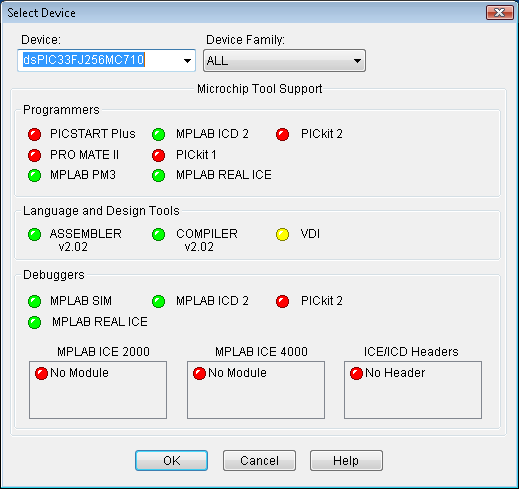
\includegraphics[
  width=6cm, bb=0 0 519 489]{images/mplab_selectdevice_dspic.png}\end{center}
\caption{Selecting the dsPIC MCU mounted on the \flex\ boards.}
\label{fig:mplab-selectdevice-dspic}
\end{figure}

\begin{figure}[htb]
\begin{center}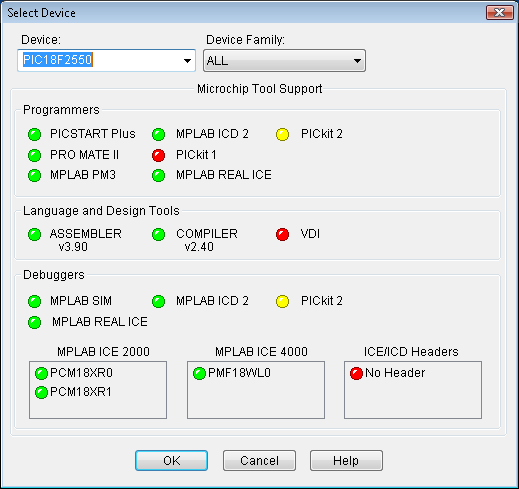
\includegraphics[
  width=6cm, bb=0 0 519 489]{images/mplab_selectdevice_pic18.png}\end{center}
\caption{Selecting the PIC18 MCU mounted on the \flex\ Full boards.}
\label{fig:mplab-selectdevice-pic18}
\end{figure}
